% GENERATED FILE - do not hand-edit.
% Source of truth: data/calculus-reviewed/c-12.json in the zenith-website repo.
% Regenerate with: python3 scripts/build_calculus_tex.py
\documentclass[11pt]{article}
\usepackage[utf8]{inputenc}
\usepackage[T1]{fontenc}
\usepackage{amsmath,amssymb}
\usepackage{graphicx}
\usepackage[margin=1in]{geometry}
\graphicspath{{../..//}}
\setlength{\parindent}{0pt}
\setlength{\parskip}{0.6em}
\begin{document}
\section*{Chapter 12: Miscellaneous Free Response Questions --- Practice Exercises C12}

\bigskip\noindent\textbf{A1.}\ A continuous, differentiable, strictly decreasing function $f$ on $[2.5,5]$ has values $\begin{array}{c|rrrrrr}x&2.5&3.2&3.5&4.0&4.6&5.0\\f(x)&7.6&5.7&4.2&3.1&2.2&1.5\end{array}$. (a) Estimate $f^{\prime}(4.0)$ and $f^{\prime}(4.8)$. (b) What does the table suggest about concavity? Explain. (c) Estimate $\int_{2.5}^5f(x)dx$ with a left Riemann sum. (d) Set up, without evaluating, a Riemann sum estimating the volume formed by rotating the region under $f$ around the $x$-axis.

\bigskip\noindent\textbf{A2.}\ The tangent to $x^2y-x=y^3-8$ at $(0,2)$ is $12y+x=24$. (a) Use it to approximate $y_0$ when $(0.3,y_0)$ lies on the curve. (b) Find the true value of $y_0$. (c) What can you conclude about the curve near $x=0$?

\bigskip\noindent\textbf{A3.}\ On $-7<x<7$, a differentiable function satisfies $f(0)=0$ and $f^{\prime}(x)=2x\sin x-e^{-x^2}+1$. (a) Describe the symmetry of $f$. (b) Find intervals where $f$ decreases. (c) Find all relative maxima of $f$ by their $x$-coordinates and justify. (d) How many inflection points does $f$ have? Justify.

\bigskip\noindent\textbf{A4.}\ Let $C$ be the first-quadrant portion of $y=\sqrt[3]{64-16x^2}$ and let $S$ be bounded by $C$ and the coordinate axes. (a) Find the tangent slope at $y=1$. (b) Find the area of $S$. (c) Find the volume generated by rotating $S$ about the $x$-axis.

\bigskip\noindent\textbf{A5.}\ Let $R$ lie on $y=x-x^2$ so that the line $OR$, with $O$ the origin, bisects the region between the curve and the $x$-axis. Set up, without solving, an integral equation for the $x$-coordinate of $R$.

\bigskip\noindent\textbf{A6.}\ Suppose $f^{\prime\prime}(x)=\sin(2^x)$ for $-1<x<3.2$. (a) Where is $f$ concave downward? Justify. (b) Find all relative minima of $f^{\prime}$ by their $x$-coordinates. (c) How many inflection points does the graph of $f^{\prime}$ have? Justify.

\bigskip\noindent\textbf{A7.}\ Let $f(x)=\cos x$ and $g(x)=x^2-1$. (a) Find all intersection points. (b) Find the area bounded by the curves.

\bigskip\noindent\textbf{A8.}\ (a) A postal employee sorts mail at these sampled rates: $\begin{array}{c|rrrrr}\text{time}&8{:}00&8{:}30&10{:}00&11{:}20&12{:}00\\\text{letters/min}&10&12&8&9&11\end{array}$. Use the trapezoidal rule to estimate the morning total. (b) A machine processes 20 letters/min; the graph shows incoming mail rates. (i) When do letters begin piling up? (ii) When is the pile largest? (iii) How many letters are then waiting? (iv) About when does the pile vanish?
\begin{center}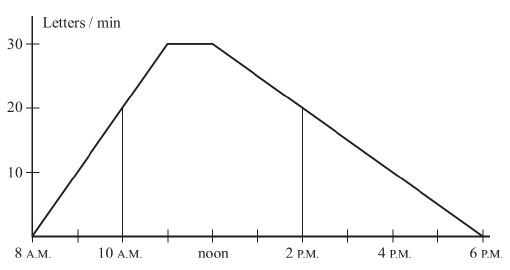
\includegraphics[width=0.6\linewidth]{data/calculus-figures/c12-a8.png}\end{center}

\bigskip\noindent\textbf{A9.}\ Let $R$ be the region bounded by $y=\sin x$ and $y=x^4$. Find (a) its area; (b) the volume of a solid with base $R$ whose cross sections perpendicular to the $x$-axis are isosceles triangles of height 3; (c) the volume when $R$ is rotated about the $x$-axis.

\bigskip\noindent\textbf{A10.}\ A water tank is the ellipsoid obtained by rotating $x^2/625+y^2/100=1$ about its minor (vertical) axis. It is 20 feet tall and 50 feet wide. (a) At 7.48 gallons per cubic foot, find capacity to the nearest thousand gallons. (b) Set up an equation, without solving, for the water depth when the tank is one-quarter full.

\bigskip\noindent\textbf{A11.}\ A sheet of metal 24 inches wide and 60 inches long is folded along its middle to make a trough with sides inclined at $60^\circ$ as shown, and ends are added. (a) Water enters at 600 in$^3$/min. How fast does the water level rise at a depth of 4 inches? (b) Instead, fold the sheet twice, making equal sides inclined at $60^\circ$. Where should the folds be to maximize the trough volume? Justify.
\begin{center}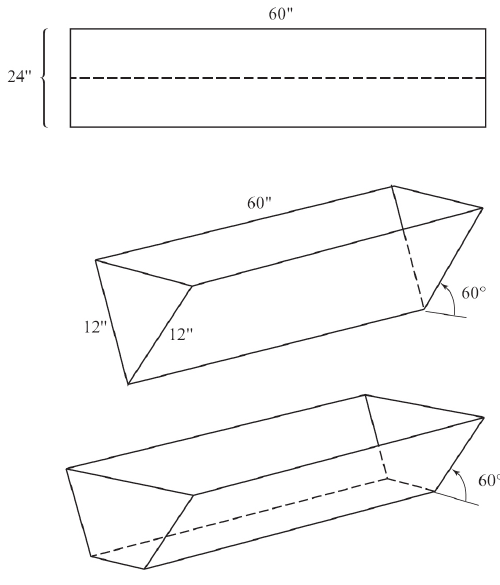
\includegraphics[width=0.6\linewidth]{data/calculus-figures/c12-a11.png}\end{center}

\bigskip\noindent\textbf{A12.}\ For $f(x)=e^{2x}(x^2-2)$: (a) Where is $f$ decreasing? (b) Does that decreasing arc reach a local or global minimum? Justify. (c) Does $f$ have a global maximum? Justify.

\bigskip\noindent\textbf{A13.}\ (a) A spherical snowball loses surface area at 10 cm$^2$/min. Find the rate of volume change when its diameter is 12 cm. (b) At that diameter its density $x$ cm from the center is $d(x)=1/(1+\sqrt x)$ g/cm$^3$. Set up, without evaluating, an integral for its mass.

\bigskip\noindent\textbf{A14.}\ (a) Numerically verify $4\arctan(1/5)-\arctan(1/239)\approx\pi/4$. (b) Use $\arctan x\approx x-x^3/3+x^5/5-x^7/7$ for $\arctan(1/5)$ and the degree-one polynomial for $\arctan(1/239)$. (c) Use these values to evaluate the expression in (a). (d) Compare this approximation for $\pi/4$ with one using $\pi/4=\arctan1$.

\bigskip\noindent\textbf{A15.}\ (a) Show that $\sum_{n=1}^{\infty}(-1)^{n+1}/\ln(n+1)$ converges. (b) How many terms suffice for a partial sum within 0.1 of its sum? (c) Classify $\sum_{n=2}^{\infty}(-1)^n/(n\ln n)$ as absolutely convergent, conditionally convergent, or divergent, and justify.

\bigskip\noindent\textbf{A16.}\ Given $dy/dt=ky(10-y)$, $y(0)=2$, and $y(2)=5$: (a) find $k$; (b) express $y$ as a function of $t$; (c) find when $y=8$; (d) describe long-term behavior.

\bigskip\noindent\textbf{A17.}\ A point $P$ moves in the first quadrant on $y=18-2x^2$, with $x=t/2$ at time $t$ seconds. (a) Find $P$ at $t=4$. (b) Find its vertical velocity there. (c) Find the rate of change of its distance from the origin at $t=4$. (d) When does it hit the $x$-axis? (e) How far does it travel in total?

\bigskip\noindent\textbf{A18.}\ A particle has $x(t)=4\arctan t$ and $y(t)=12t/(t^2+1)$ for $t\ge0$. (a) Sketch its path and direction. (b) Find the time of its highest point and justify. (c) Find that point and sketch the velocity vector there. (d) Describe its long-term behavior.

\bigskip\noindent\textbf{A19.}\ Let $R$ be bounded by $r=2+\cos2\theta$, as shown. (a) Find the dimensions of the smallest containing rectangle with sides parallel to the coordinate axes. (b) Find the area of $R$.
\begin{center}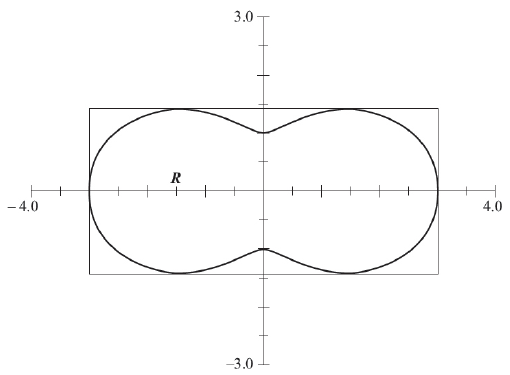
\includegraphics[width=0.6\linewidth]{data/calculus-figures/c12-a19.png}\end{center}

\bigskip\noindent\textbf{A20.}\ (a) For what positive $x$ does $f(x)=\sum_{n=1}^{\infty}(-1)^{n+1}x^n/\ln(n+1)$ converge? (b) How many terms suffice to estimate $f(0.5)$ within 0.01? (c) Would using the same number of terms at $x=-0.5$ be more accurate, less accurate, or equally accurate? Explain.

\bigskip\noindent\textbf{A21.}\ Researchers introduce 100 trout into a lake and model their population $F$ after $m$ months by $dF/dm=0.0002F(600-F)$. (a) At what population is growth fastest? (b) Solve for $F(m)$. (c) When is the population growing fastest?

\bigskip\noindent\textbf{B1.}\ Sketch $y=f(x)$ satisfying all these conditions: (a) $f^{\prime}(-1)=f^{\prime}(1)=0$; (b) for $x<-1$, $f^{\prime}>0$, $f^{\prime\prime}<0$; (c) for $-1<x<0$, $f^{\prime}>0$, $f^{\prime\prime}>0$; (d) for $0<x<1$, $f^{\prime}>0$, $f^{\prime\prime}<0$; (e) for $x>1$, $f^{\prime}<0$, $f^{\prime\prime}<0$.

\bigskip\noindent\textbf{B2.}\ The graph of $f^{\prime}$ on $[-3,9]$ is shown, with horizontal tangents at 2 and 4 and a corner at 6. (a) Is $f$ continuous? Explain. (b) Find local minima of $f$ by their $x$-coordinates. (c) Find local maxima. (d) Where is the absolute maximum? (e) Find all inflection points by their $x$-coordinates. Justify each answer.
\begin{center}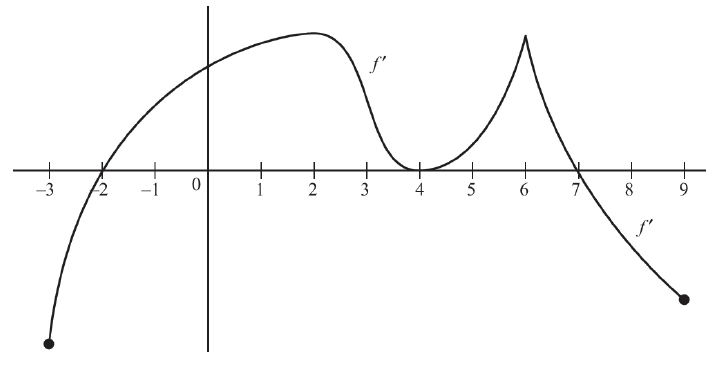
\includegraphics[width=0.6\linewidth]{data/calculus-figures/c12-b2.png}\end{center}

\bigskip\noindent\textbf{B3.}\ Find the area of the largest rectangle with sides parallel to the coordinate axes inscribed between $f(x)=8-2x^2$ and $g(x)=x^2-4$.

\bigskip\noindent\textbf{B4.}\ Given the displayed graph of $f(x)$, sketch the graph of $f^{\prime}(x)$.
\begin{center}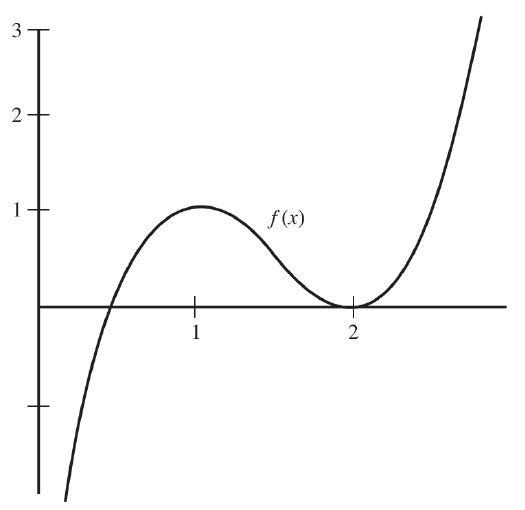
\includegraphics[width=0.6\linewidth]{data/calculus-figures/c12-b4.png}\end{center}

\bigskip\noindent\textbf{B5.}\ A cube contracts so its surface area decreases at 72 in$^2$/sec. Find the rate of volume change when its surface area is 54 ft$^2$.

\bigskip\noindent\textbf{B6.}\ A square is inscribed in a circle of radius $a$ as shown. Find the volume formed by rotating the region inside the circle and outside the square about a diagonal of the square.
\begin{center}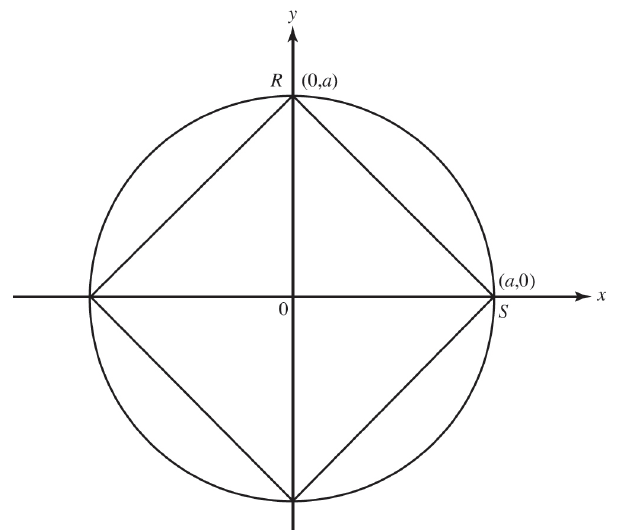
\includegraphics[width=0.6\linewidth]{data/calculus-figures/c12-b6.png}\end{center}

\bigskip\noindent\textbf{B7.}\ (a) Sketch the first-quadrant region bounded above by $y=x+4$, below by $y=4-x$, and on the right by $y=x^2+2$. (b) Find its area.

\bigskip\noindent\textbf{B8.}\ The graph shows an index of food production in South Asia. (a) During which intervals did production decrease? (b) When did the rate of change of production increase? (c) When did the increase in production accelerate?
\begin{center}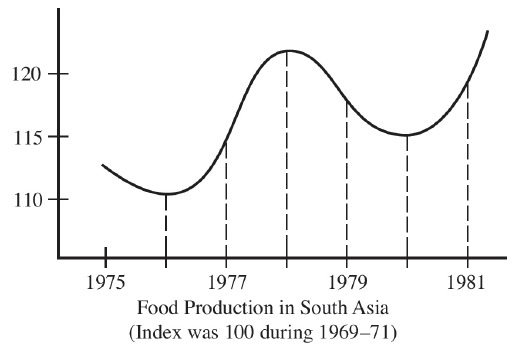
\includegraphics[width=0.6\linewidth]{data/calculus-figures/c12-b8.png}\end{center}

\bigskip\noindent\textbf{B9.}\ A particle moves along a line with acceleration $a=-2v$. (a) Find $v(t)$ given $v(0)=20$. (b) Find the distance traveled while its velocity decreases from 20 to 5.

\bigskip\noindent\textbf{B10.}\ An isosceles triangle $AOB$ is inscribed in the region below $y=27-x^2$ and above the $x$-axis, with vertex $O=(0,0)$ and base $AB$ parallel to the $x$-axis. Find its maximum area.

\bigskip\noindent\textbf{B11.}\ Newton’s law says the rate of temperature change is proportional to the difference between an object’s temperature and its surroundings. At 9:00 P.M., milk is $40^\circ$ in a $68^\circ$ room; at 9:03 it is $43^\circ$, and a friend calls with a calculus problem. If milk above $60^\circ$ is unacceptable, how many minutes from the call do you have, to the nearest minute?

\bigskip\noindent\textbf{B12.}\ An even function $h$ is continuous on $[-4,4]$ and has these properties: $\begin{array}{c|ccc}x&h&h^{\prime}&h^{\prime\prime}\\0&-&0&+\\0<x<1&-&+&+\\1&0&+&0\\1<x<2&+&+&-\\2&+&0&0\\2<x<3&+&+&+\\3&+&\text{undefined}&\text{undefined}\\3<x<4&+&-&-\end{array}$. Sketch a possible graph.

\bigskip\noindent\textbf{B13.}\ (a) Find the Maclaurin series for $f(x)=\ln(1+x)$. (b) Find its radius of convergence. (c) Use its first five terms to approximate $\ln(1.2)$. (d) Bound the error and justify.

\bigskip\noindent\textbf{B14.}\ The cycloid is $x=\theta-\sin\theta$, $y=1-\cos\theta$. (a) Find its slope at $\theta=2\pi/3$. (b) Find the tangent equation at that point.

\bigskip\noindent\textbf{B15.}\ Find the area enclosed in common by the polar curves $r=4\sin\theta$ and $r=4\cos\theta$.

\bigskip\noindent\textbf{B16.}\ (a) Find the fourth-degree Taylor polynomial about 0 for $\cos x$. (b) Use it to approximate $\int_0^1\cos x\,dx$. (c) Bound the approximation error and justify.

\bigskip\noindent\textbf{B17.}\ A particle moves on $y^3=2x+1$, with distance from the $x$-axis increasing at 2 units/sec, starting at $(0,1)$ when $t=0$. (a) Find parametric equations for $t\ge0$. (b) Find the acceleration magnitude at $t=1$.

\bigskip\noindent\textbf{B18.}\ Find the area enclosed in common by $r=2-\cos\theta$ and $r=3\cos\theta$.

\end{document}
